\documentclass[12pt,twoside]{article}

\newcommand{\reporttitle}{Numerical Analysis of ODEs using Matlab}
\newcommand{\reportauthor}{Mwana}
\newcommand{\reportauthora}{Aufar}
\newcommand{\reportauthorb}{Zihan}
\newcommand{\reportauthorc}{Calvin}
\newcommand{\reportauthord}{Yann Herklotz}
\newcommand{\reporttype}{Mathematics Coursework}
\newcommand{\email}{}
\newcommand{\emaila}{apl115@ic.ac.uk}
\newcommand{\emailb}{}
\newcommand{\emailc}{}
\newcommand{\emaild}{ymh15@ic.ac.uk}

% include files that load packages and define macros
%%%%%%%%%%%%%%%%%%%%%%%%%%%%%%%%%%%%%%%%%
% University Assignment Title Page 
% LaTeX Template
% Version 1.0 (27/12/12)
%
% This template has been downloaded from:
% http://www.LaTeXTemplates.com
%
% Original author:
% WikiBooks (http://en.wikibooks.org/wiki/LaTeX/Title_Creation)
%
% License:
% CC BY-NC-SA 3.0 (http://creativecommons.org/licenses/by-nc-sa/3.0/)
% 
% Instructions for using this template:
% This title page is capable of being compiled as is. This is not useful for 
% including it in another document. To do this, you have two options: 
%
% 1) Copy/paste everything between \begin{document} and \end{document} 
% starting at \begin{titlepage} and paste this into another LaTeX file where you 
% want your title page.
% OR
% 2) Remove everything outside the \begin{titlepage} and \end{titlepage} and 
% move this file to the same directory as the LaTeX file you wish to add it to. 
% Then add \input{./title_page_1.tex} to your LaTeX file where you want your
% title page.
%
%----------------------------------------------------------------------------------------
%	PACKAGES AND OTHER DOCUMENT CONFIGURATIONS
%----------------------------------------------------------------------------------------
\usepackage{ifxetex}
\usepackage{textpos}
\usepackage{natbib}
\usepackage{kpfonts}
\usepackage[a4paper,hmargin=2.8cm,vmargin=2.0cm,includeheadfoot]{geometry}
\usepackage{ifxetex}
\usepackage{stackengine}
\usepackage{tabularx,longtable,multirow,subfigure,caption}%hangcaption
\usepackage{fncylab} %formatting of labels
\usepackage{fancyhdr}
\usepackage{color}
\usepackage[tight,ugly]{units}
\usepackage{url}
\usepackage{float}
\usepackage[english]{babel}
\usepackage{amsmath}
\usepackage{graphicx}
\usepackage[colorinlistoftodos]{todonotes}
\usepackage{dsfont}
\usepackage{epstopdf} % automatically replace .eps with .pdf in graphics
\usepackage{natbib}
\usepackage{backref}
\usepackage{array}
\usepackage{latexsym}
\usepackage{etoolbox}

\usepackage{enumerate} % for numbering with [a)] format 



\ifxetex
\usepackage{fontspec}
\setmainfont[Scale=.8]{OpenDyslexic-Regular}
\else
\usepackage[pdftex,pagebackref,hypertexnames=false,colorlinks]{hyperref} % provide links in pdf
\hypersetup{pdftitle={},
  pdfsubject={}, 
  pdfauthor={\reportauthor},
  pdfkeywords={}, 
  pdfstartview=FitH,
  pdfpagemode={UseOutlines},% None, FullScreen, UseOutlines
  bookmarksnumbered=true, bookmarksopen=true, colorlinks,
    citecolor=black,%
    filecolor=black,%
    linkcolor=black,%
    urlcolor=black}
\usepackage[all]{hypcap}
\fi

\usepackage{tcolorbox}

% various theorems
\usepackage{ntheorem}
\theoremstyle{break}
\newtheorem{lemma}{Lemma}
\newtheorem{theorem}{Theorem}
\newtheorem{remark}{Remark}
\newtheorem{definition}{Definition}
\newtheorem{proof}{Proof}

% example-environment
\newenvironment{example}[1][]
{ 
\vspace{4mm}
\noindent\makebox[\linewidth]{\rule{\hsize}{1.5pt}}
\textbf{Example #1}\\
}
{ 
\noindent\newline\makebox[\linewidth]{\rule{\hsize}{1.0pt}}
}



%\renewcommand{\rmdefault}{pplx} % Palatino
% \renewcommand{\rmdefault}{put} % Utopia

\ifxetex
\else
\renewcommand*{\rmdefault}{bch} % Charter
\renewcommand*{\ttdefault}{cmtt} % Computer Modern Typewriter
%\renewcommand*{\rmdefault}{phv} % Helvetica
%\renewcommand*{\rmdefault}{iwona} % Avant Garde
\fi

\setlength{\parindent}{0em}  % indentation of paragraph

\setlength{\headheight}{14.5pt}
\pagestyle{fancy}
\fancyfoot[ER,OL]{\thepage}%Page no. in the left on
                                %odd pages and on right on even pages
\fancyfoot[OC,EC]{\sffamily }
\renewcommand{\headrulewidth}{0.1pt}
\renewcommand{\footrulewidth}{0.1pt}
\captionsetup{margin=10pt,font=small,labelfont=bf}


%--- chapter heading

\def\@makechapterhead#1{%
  \vspace*{10\p@}%
  {\parindent \z@ \raggedright %\sffamily
        %{\Large \MakeUppercase{\@chapapp} \space \thechapter}
        %\\
        %\hrulefill
        %\par\nobreak
        %\vskip 10\p@
    \interlinepenalty\@M
    \Huge \bfseries 
    \thechapter \space\space #1\par\nobreak
    \vskip 30\p@
  }}

%---chapter heading for \chapter*  
\def\@makeschapterhead#1{%
  \vspace*{10\p@}%
  {\parindent \z@ \raggedright
    \sffamily
    \interlinepenalty\@M
    \Huge \bfseries  
    #1\par\nobreak
    \vskip 30\p@
  }}
  



% %%%%%%%%%%%%% boxit
\def\Beginboxit
   {\par
    \vbox\bgroup
	   \hrule
	   \hbox\bgroup
		  \vrule \kern1.2pt %
		  \vbox\bgroup\kern1.2pt
   }

\def\Endboxit{%
			      \kern1.2pt
		       \egroup
		  \kern1.2pt\vrule
		\egroup
	   \hrule
	 \egroup
   }	

\newenvironment{boxit}{\Beginboxit}{\Endboxit}
\newenvironment{boxit*}{\Beginboxit\hbox to\hsize{}}{\Endboxit}



\allowdisplaybreaks

\makeatletter
\newcounter{elimination@steps}
\newcolumntype{R}[1]{>{\raggedleft\arraybackslash$}p{#1}<{$}}
\def\elimination@num@rights{}
\def\elimination@num@variables{}
\def\elimination@col@width{}
\newenvironment{elimination}[4][0]
{
    \setcounter{elimination@steps}{0}
    \def\elimination@num@rights{#1}
    \def\elimination@num@variables{#2}
    \def\elimination@col@width{#3}
    \renewcommand{\arraystretch}{#4}
    \start@align\@ne\st@rredtrue\m@ne
}
{
    \endalign
    \ignorespacesafterend
}
\newcommand{\eliminationstep}[2]
{
    \ifnum\value{elimination@steps}>0\leadsto\quad\fi
    \left[
        \ifnum\elimination@num@rights>0
            \begin{array}
            {@{}*{\elimination@num@variables}{R{\elimination@col@width}}
            |@{}*{\elimination@num@rights}{R{\elimination@col@width}}}
        \else
            \begin{array}
            {@{}*{\elimination@num@variables}{R{\elimination@col@width}}}
        \fi
            #1
        \end{array}
    \right]
    & 
    \begin{array}{l}
        #2
    \end{array}
    &%                                    moved second & here
    \addtocounter{elimination@steps}{1}
}
\makeatother

%% Fast macro for column vectors
\makeatletter  
\def\colvec#1{\expandafter\colvec@i#1,,,,,,,,,\@nil}
\def\colvec@i#1,#2,#3,#4,#5,#6,#7,#8,#9\@nil{% 
  \ifx$#2$ \begin{bmatrix}#1\end{bmatrix} \else
    \ifx$#3$ \begin{bmatrix}#1\\#2\end{bmatrix} \else
      \ifx$#4$ \begin{bmatrix}#1\\#2\\#3\end{bmatrix}\else
        \ifx$#5$ \begin{bmatrix}#1\\#2\\#3\\#4\end{bmatrix}\else
          \ifx$#6$ \begin{bmatrix}#1\\#2\\#3\\#4\\#5\end{bmatrix}\else
            \ifx$#7$ \begin{bmatrix}#1\\#2\\#3\\#4\\#5\\#6\end{bmatrix}\else
              \ifx$#8$ \begin{bmatrix}#1\\#2\\#3\\#4\\#5\\#6\\#7\end{bmatrix}\else
                 \PackageError{Column Vector}{The vector you tried to write is too big, use bmatrix instead}{Try using the bmatrix environment}
              \fi
            \fi
          \fi
        \fi
      \fi
    \fi
  \fi 
}  
\makeatother

\robustify{\colvec}

%%% Local Variables: 
%%% mode: latex
%%% TeX-master: "notes"
%%% End: 
 % various packages needed for maths etc.
% quick way of adding a figure
\newcommand{\fig}[3]{
 \begin{center}
 \scalebox{#3}{\includegraphics[#2]{#1}}
 \end{center}
}

%\newcommand*{\point}[1]{\vec{\mkern0mu#1}}
\newcommand{\ci}[0]{\perp\!\!\!\!\!\perp} % conditional independence
\newcommand{\point}[1]{{#1}} % points 
\renewcommand{\vec}[1]{{\boldsymbol{{#1}}}} % vector
\newcommand{\mat}[1]{{\boldsymbol{{#1}}}} % matrix
\newcommand{\R}[0]{\mathds{R}} % real numbers
\newcommand{\Z}[0]{\mathds{Z}} % integers
\newcommand{\N}[0]{\mathds{N}} % natural numbers
\newcommand{\nat}[0]{\mathds{N}} % natural numbers
\newcommand{\Q}[0]{\mathds{Q}} % rational numbers
\ifxetex
\newcommand{\C}[0]{\mathds{C}} % complex numbers
\else
\newcommand{\C}[0]{\mathds{C}} % complex numbers
\fi
\newcommand{\tr}[0]{\text{tr}} % trace
\renewcommand{\d}[0]{\mathrm{d}} % total derivative
\newcommand{\inv}{^{-1}} % inverse
\newcommand{\id}{\mathrm{id}} % identity mapping
\renewcommand{\dim}{\mathrm{dim}} % dimension
\newcommand{\rank}[0]{\mathrm{rk}} % rank
\newcommand{\determ}[1]{\mathrm{det}(#1)} % determinant
\newcommand{\scp}[2]{\langle #1 , #2 \rangle}
\newcommand{\kernel}[0]{\mathrm{ker}} % kernel/nullspace
\newcommand{\img}[0]{\mathrm{Im}} % image
\newcommand{\idx}[1]{{(#1)}}
\DeclareMathOperator*{\diag}{diag}
\newcommand{\E}{\mathds{E}} % expectation
\newcommand{\var}{\mathds{V}} % variance
\newcommand{\gauss}[2]{\mathcal{N}\big(#1,\,#2\big)} % gaussian distribution N(.,.)
\newcommand{\gaussx}[3]{\mathcal{N}\big(#1\,|\,#2,\,#3\big)} % gaussian distribution N(.|.,.)
\newcommand{\gaussBig}[2]{\mathcal{N}\left(#1,\,#2\right)} % see above, but with brackets that adjust to the height of the arguments
\newcommand{\gaussxBig}[3]{\mathcal{N}\left(#1\,|\,#2,\,#3\right)} % see above, but with brackets that adjust to the height of the arguments
\DeclareMathOperator{\cov}{Cov} % covariance (matrix) 
\ifxetex
\renewcommand{\T}[0]{^\top} % transpose
\else
\newcommand{\T}[0]{^\top}
\fi
% matrix determinant
\newcommand{\matdet}[1]{
\left|
\begin{matrix}
#1
\end{matrix}
\right|
}



%%% various color definitions
\definecolor{darkgreen}{rgb}{0,0.6,0}

\newcommand{\blue}[1]{{\color{blue}#1}}
\newcommand{\red}[1]{{\color{red}#1}}
\newcommand{\green}[1]{{\color{darkgreen}#1}}
\newcommand{\orange}[1]{{\color{orange}#1}}
\newcommand{\magenta}[1]{{\color{magenta}#1}}
\newcommand{\cyan}[1]{{\color{cyan}#1}}


% redefine emph
\renewcommand{\emph}[1]{\blue{\bf{#1}}}

% place a colored box around a character
\gdef\colchar#1#2{%
  \tikz[baseline]{%
  \node[anchor=base,inner sep=2pt,outer sep=0pt,fill = #2!20] {#1};
    }%
}%
 % short-hand notation and macros


%%%%%%%%%%%%%%%%%%%%%%%%%%%%

\begin{document}
% front page
% Last modification: 2016-09-29 (Marc Deisenroth)
\begin{titlepage}

\newcommand{\HRule}{\rule{\linewidth}{0.5mm}} % Defines a new command for the horizontal lines, change thickness here


%----------------------------------------------------------------------------------------
%	LOGO SECTION
%----------------------------------------------------------------------------------------


\includegraphics[width = 4cm]{./figures/imperial}\\[0.5cm] 

\begin{center} % Center remainder of the page

%----------------------------------------------------------------------------------------
%	HEADING SECTIONS
%----------------------------------------------------------------------------------------
\textsc{\LARGE \reporttype}\\[1.5cm] 
\textsc{\Large Imperial College London}\\[0.5cm] 
\textsc{\large Department of Electrical and Electronic Engineering}\\[0.5cm] 
%----------------------------------------------------------------------------------------
%	TITLE SECTION
%----------------------------------------------------------------------------------------

\HRule \\[0.4cm]
{ \huge \bfseries \reporttitle}\\ % Title of your document
\HRule \\[1.5cm]
\end{center}
%----------------------------------------------------------------------------------------
%	AUTHOR SECTION
%----------------------------------------------------------------------------------------

%\begin{minipage}{0.4\hsize}
\begin{flushleft} \large
\textit{Authors:}\\
\reportauthor~(email: \email) \\% Your name 
\reportauthora~(email: \emaila) \\% Your name
\reportauthorb~(email: \emailb) \\% Your name
\reportauthorc~(email: \emailc) \\% Your name
\reportauthord~(email: \emaild) % Your name
\end{flushleft}
\vspace{2cm}
\makeatletter
Date: \@date 

\vfill % Fill the rest of the page with whitespace



\makeatother


\end{titlepage}



\tableofcontents

%%%%%%%%%%%%%%%%%%%%%%%%%%%% Main document


%%%%%%%%%%%%%%%%%%%%%%%%%%%% Introduction

\newpage
\section{Introduction}

%%%%%%%%%%%%%%%%%%%%%%%%%%%% Part 1

\newpage
\section{RL Circuit}

%%%%%%%%%%%%%%%%%%%%%%%%%%%% Part 2: Exercise 3: RLC Circuit

\newpage
\section{RLC Circuit}

\subsection{RLC Circuit Equation}

An RLC circuit consists of a resistor, capacitor and an inductor. For the purpose of this example, we have a series RLC circuit, as shown in the figure below.

\begin{figure}[h]
\centering
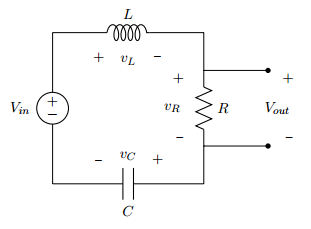
\includegraphics[width = 8cm]{./figures/RLC.PNG}\\[0.01cm]
\caption{Series RLC Circuit}
\end{figure}

By applying Kirchoff's Voltage Law for each of the three components of the circuit, we can obtain the differential equation representing the circuit.

\[
V_{R} + V_{L} + V_{C} = V_{in}(t)
\]

\[
L \frac{d}{dt}i_{L}(t) + R i_{L}(t) + \frac{1}{C} \int_0^t i_{L}(\tau) \,d\tau = V_{in}(t)
\]

\[
L \frac{d^2}{dt^2} q_{C}(t) + R \frac{d}{dt} q_{C}(t) + \frac{1}{C}  q_{C}(t) = V_{in}(t)
\]

We assume that the capacitor is pre-charged at time t = 0, with q$_{\text{C}}$(0) = 500nC. We also assume that no current flows through the inductor at time t = 0, so i$_{\text{L}}$(0) = $\frac{d}{dt}q_{\text{C}}$(0) = 0A.

We were also given the values of resistances, capacitance and inductance of the components in the circuit:

\begin{center}
R = 250$\Omega$, C = 3$\mu$F, L = 650mH 
\end{center}

\subsection{Runge-Kutta and Coupled Equations}
\subsubsection{Runge-Kutta}
Runge-Kutta 4th order method is a numerical technique used to solve ordinary differential equations of the form $\frac{dy}{dx} = f(x,y)$, where y(0) = y$_{\text{0}}$. Therefore, we can only use it to solve first order ordinary differential equations.

\subsubsection{Coupled Equations}
In order to solve the RLC equation derived earlier, we need to rewrite the equation in a \textit{coupled} form. We take the equation:
\[
L \frac{d^2}{dt^2} q_{C}(t) + R \frac{d}{dt} q_{C}(t) + \frac{1}{C}  q_{C}(t) = V_{in}(t)
\]

By letting  y = $\frac{d}{dt}q_{C}(t)$ = $\dot{q}$ and  = $\frac{d^2}{dt^2}q_{C}(t)$ = $\ddot{q}$, we can do:

\[
L\ddot{q} + R\dot{q} + \frac{1}{C}q = V_{in}
\]

\[
L
\]

\subsection{Matlab Script}

\subsubsection{Runge-Kutta 3/8}


%%%%%%%%%%%%%%%%%%%%%%%%%%%% Part 3: Exercise 4: Finite Differences for PDE

\newpage
\section{Finite Differences for PDE}

\subsection{1-D Heat Equation}

The 1-D heat equation \\

\[
\frac{\partial y}{\partial t} = \frac{\partial ^2 y}{\partial x^2},\quad 0 < x < 1,\quad t > 0
\]\\

with zero boundary conditions \( y(0, t) = y(1, t) = 0 \) and initial conditions \\
\( y(x, 0) = y_0(x) \) can be solved numerically using the finite difference method.


\subsection{Method}

The finite difference method consists of approximating a differential equation using difference equations. As the 
1-D heat equation has depends on \( x \) and \( t \) we can use the finite difference method to approximate the heat
equation when \( t = 0 \) and then increment \( t \) to get the heat equation as it changes over time. 


\subsection{Matlab Script}

There were certain aspects of the finite difference method that had to be considered when implementing it in Matlab.
We had to find the right values that would give the precision that we wanted and display the results properly. We used a
\( (N+1) \times (m+1) \) matrix to store all the results from the finite difference method. The matrix has 1 added to \( N \) and
\( m \) because Matlab starts its index at 1 and we want to go from \( 0..N \) and from \( 0..m \).

\subsubsection{Boundary Conditions}

First of all, we had to find a way of adding the boundary conditions that we wanted to the the finite differences method
and still be able to change these easily, because we had to test different ones. We solved this by writing a function that enabled us
to choose the function that we wanted to use as a boundary condition. To this Matlab function we could then easily add more functions
that could then be used as a boundary condition and we could easily test these boundary conditions. The boundary conditions 
can also be expressed as \( U_0^m,\ U_N^m \). This means we just have to set all the numbers at index 1 and index \( N+1 \) to 
be equal to the initial condition. This way we can also set the initial condition to be a different constant, or even an equation that
changes with time.


\subsubsection{Central Algorithm}

The main part of the finite difference method is the central algorithm, as this is the algorithm that is derived from the approximations
of the initial differential equation that we want to solve. 

The central algorithm for the 1-D heat equation is

\[
U_{j}^{m+1} =\ v U_{j-1}^{m} + (1 - 2 v) U_{j}^{m} + v U_{j+1}^{m}
\]\\

We want to implement this algorithm for every value of from \( 0..m \) and every value from \( 0..N \). This can be done by using two 
for loops that will iterate over the matrix, and for every \( m \), to get \( m+1 \) we will pass the required values to the equation.

As we have a matrix with all the previous values that have been calculated, we can use it to get the values of \( U_{j-1}^m,\ U_j^m,\ 
U_{j+1}^m \) directly from the matrix. 


\subsubsection{Choosing Constants}

\subsubsection{Plotting Results}


\subsection{Solving the Heat Equation}

\subsubsection{Tent Function Initial Condition}

\subsubsection{Sinusoidal Function}


\section{Bonus}


\end{document}
